
\setlength\fboxrule{0pt}
\begin{center}
	\fcolorbox{white}{white!100}{
		\fbox{



	\begin{minipage}{13em}
	\begin{center}      	
		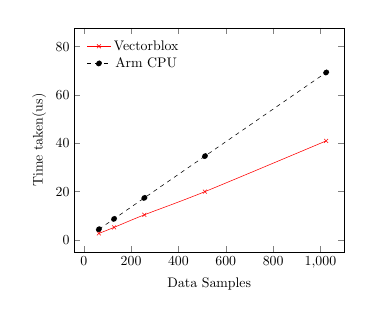
\begin{tikzpicture}[scale=0.5]
		\begin{axis}[
		xlabel=Data Samples,
		enlarge y limits = true,
		ylabel=Time taken(us),
		ymax = 80,
		xmax = 1100,
		legend pos=north west,
		legend style={draw=none}
		]
		\addplot [smooth,mark=x,red] plot coordinates {
			(64,     2.7)
			(128,    5.2)
			(256,    10.4)
			(512,    20)
			(1024,   41)			
		};
		\addplot [smooth,mark=*,dashed] plot coordinates {
			(64,     4.43)
			(128,    8.71)
			(256,    17.4)
			(512,    34.69)
			(1024,   69.30)
			
		};
		\legend{Vectorblox\\Arm CPU\\}
		\end{axis}
		\end{tikzpicture}
	\end{center}  
	\tiny  
	Vectorblox C API Implementation in Comparison with naive C Implementation on ARM CPU.
	\end{minipage}

	\hspace{1em}
	\begin{minipage}{13em}
	\begin{center}      				
	 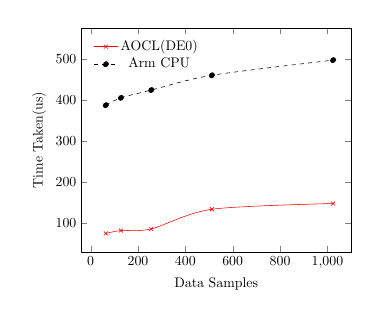
\begin{tikzpicture}[scale=0.5]
	 \begin{axis}[
	 xlabel=Data Samples,
	 ylabel=Time Taken(us),
	 enlarge y limits = true,
	 ymax = 530,
	 xmax = 1100,
	 legend pos=north west,
	 legend style={draw=none}
	 ]
	 \addplot [smooth,mark=x,red] plot coordinates {
			(64,     74)
			(128,    81)
			(256,    85)
			(512,    133)
			(1024,   147)			
		};
		\addplot [smooth,mark=*,dashed] plot coordinates {
			(64,     387)
			(128,    405)
			(256,    424)
			(512,    460)
			(1024,   497)
			
		};
	 \legend{AOCL(DE0)\\Arm CPU\\}
	 \end{axis}
	 \end{tikzpicture}
	\end{center}
	\tiny 
	OpenCL Implementation Timing Comparison between ARM CPU and AOCL FPGA Implementation.   					
	\end{minipage}
					
		}
	}
\end{center}


